\chapter{Medindo tudo}
\markboth{Módulo 4}{}

\enlargethispage{3\baselineskip}

\section*{Habilidades do SAEB}

\begin{itemize}
\item Reconhecer a unidade de medida ou o instrumento mais apropriado para
medições de comprimento, área, massa, tempo, capacidade ou temperatura.

\item Estimar/inferir medida de comprimento, capacidade ou massa de objetos,
utilizando unidades de medida convencionais ou não ou medir comprimento,
capacidade ou massa de objetos.

\item Explicar que o resultado de uma medida depende da unidade de medida
utilizada.

\item Resolver problemas que envolvam medidas de grandezas (comprimento,
massa, tempo e capacidade) em que haja conversões entre as unidades mais
usuais.

\item Determinar o horário de início, o horário de término ou a duração de
um acontecimento.
\end{itemize}

\subsection{Habilidades da BNCC}

\begin{itemize}
\item EF03MA19, EF03MA20.
\end{itemize}



%\conteudo{
%\noindent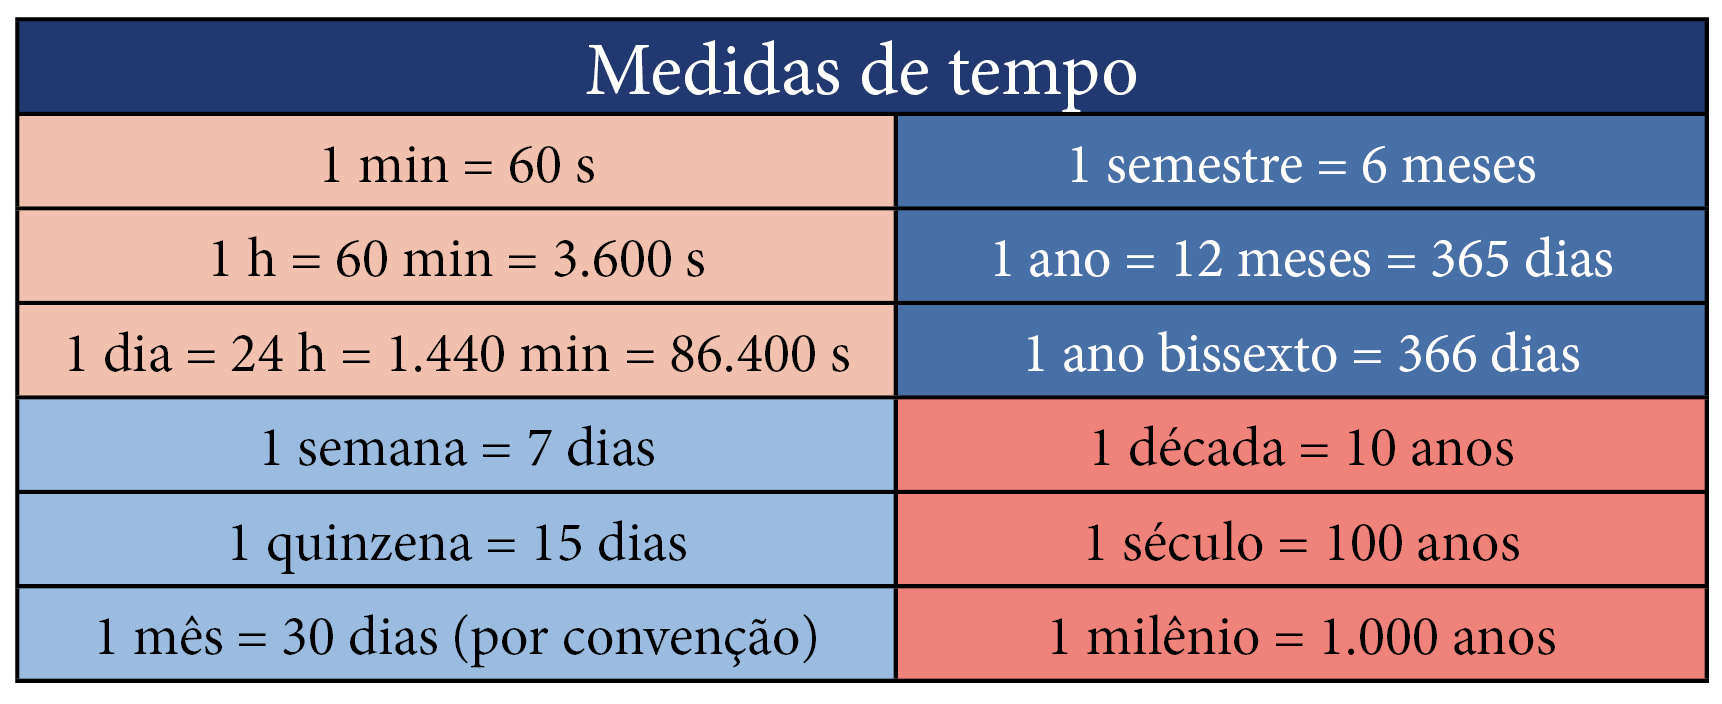
\includegraphics[width=\textwidth]{./media/image39.png}
%} 

\conteudo{
Unidade de medida é uma referência estabelecida para que todos possam medir e comparar grandezas físicas, obtendo os mesmos resultados. Por exemplo, hora, período, dia, semana, mês, ano, década, século, milênio são unidades de medida de tempo.

Observe a tabela a seguir para lembrar das unidades de medida de comprimento, massa e volume.    

\noindent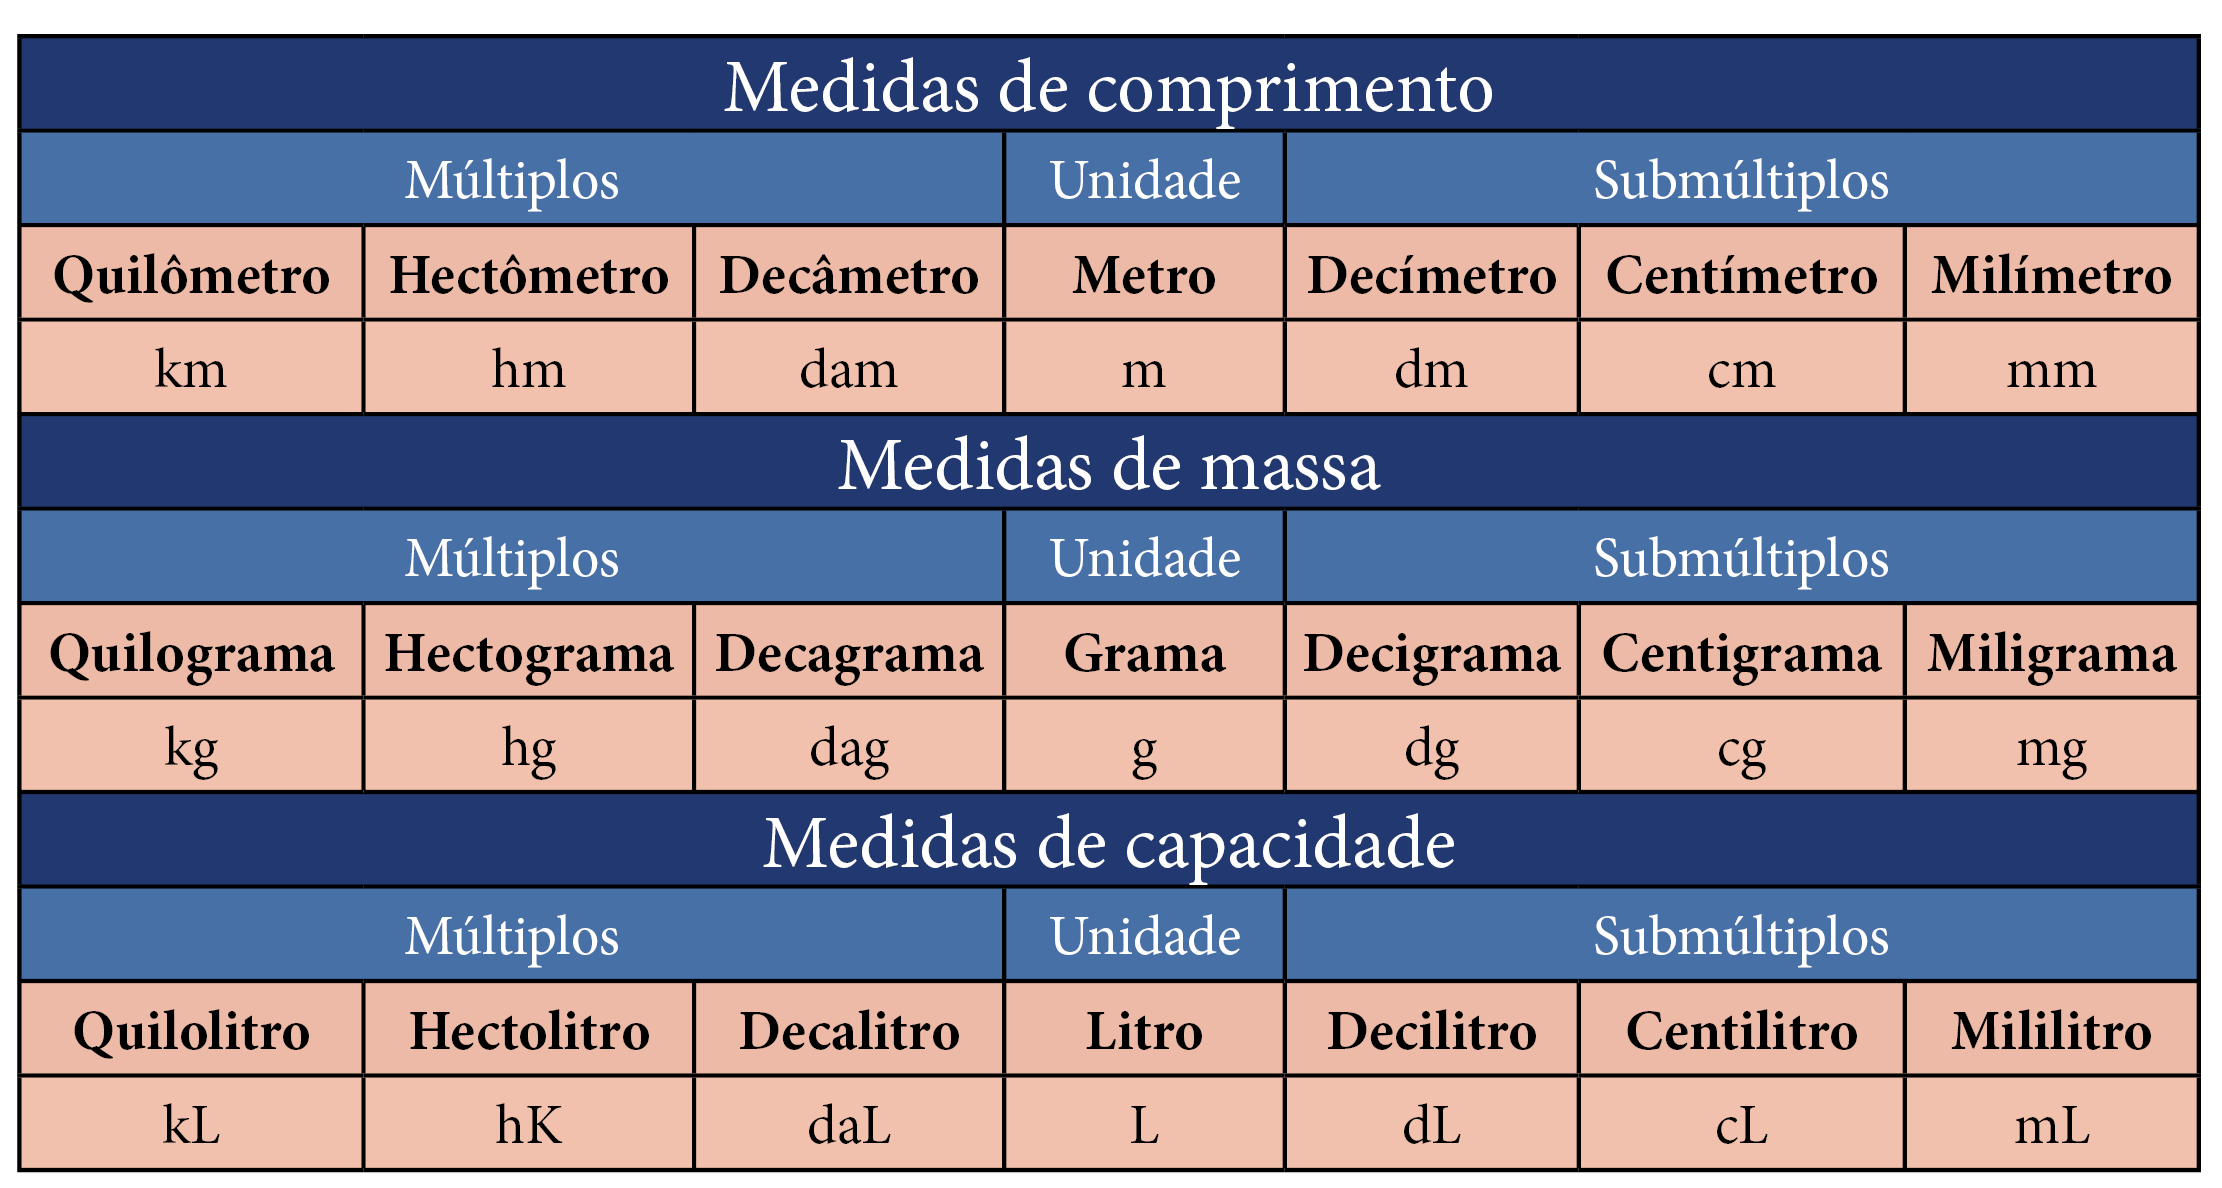
\includegraphics[width=\textwidth]{./media/image38.png}
}

\section*{Atividades}

\num{1} A régua é utilizada para medir comprimento.

\begin{figure}[htpb!]
\centering
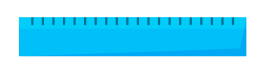
\includegraphics[width=.7\textwidth]{./media/image41a.png}
\end{figure}

\begin{escolha}
\item Escreva o nome de dois objetos da sala de aula que você acredita
  medirem menos de 1 metro.
\reduline{Resposta pessoal.\hfill}
\linhas{2}

\item Escreva o nome de dois objetos da sala de aula que você acredita
  medirem mais de 1 metro.
\reduline{Resposta pessoal.\hfill}
\linhas{2}
\end{escolha}

\num{2} Utilize sua régua para responder aos itens a seguir.

\begin{escolha}
\item Quantos centímetros tem o comprimento da sua borracha?
\reduline{Resposta pessoal.\hfill}

\item Qual é a largura, em centímetros, da carteira que você utiliza na sala de aula?
\reduline{Resposta pessoal.\hfill}

\item Qual é o comprimento, em centímetros, do seu lápis?
\reduline{Resposta pessoal.\hfill}

\item Qual é a altura aproximada de um dos seus colegas?
\reduline{Resposta pessoal.\hfill}
\end{escolha}

\num{3} Relacione a primeira com a segunda coluna, levando em conta qual é valor que 
pode corresponder à cada medida.


\begin{multicols}{2}\parindent=0em
A. Altura aproximada\\
de uma porta\bigskip

B. Comprimento aproximado\\
de um lápis\bigskip

C. Comprimento médio\\
de um quarteirão\bigskip

D. Comprimento aproximado de\\
uma quadra de basquete

\columnbreak

(\hspace{2em}) 20 cm\bigskip

(\hspace{2em}) 90 m\bigskip

(\hspace{2em}) 30 m\bigskip

(\hspace{2em}) 2 m
\end{multicols}


\coment{Resposta: B, C, D, A.}

\pagebreak

\num{4} Complete a frase com o número que representa quanto mede cada um dos
objetos indicados a seguir.

\begin{escolha}

\item O lápis mede \reduline{9 cm.\hfill}

\begin{center}
\noindent
\includegraphics[width=0.8\textwidth]{./media/image42.png}
\end{center}

\item A borracha mede \reduline{6 cm.\hfill}

\begin{center}
\noindent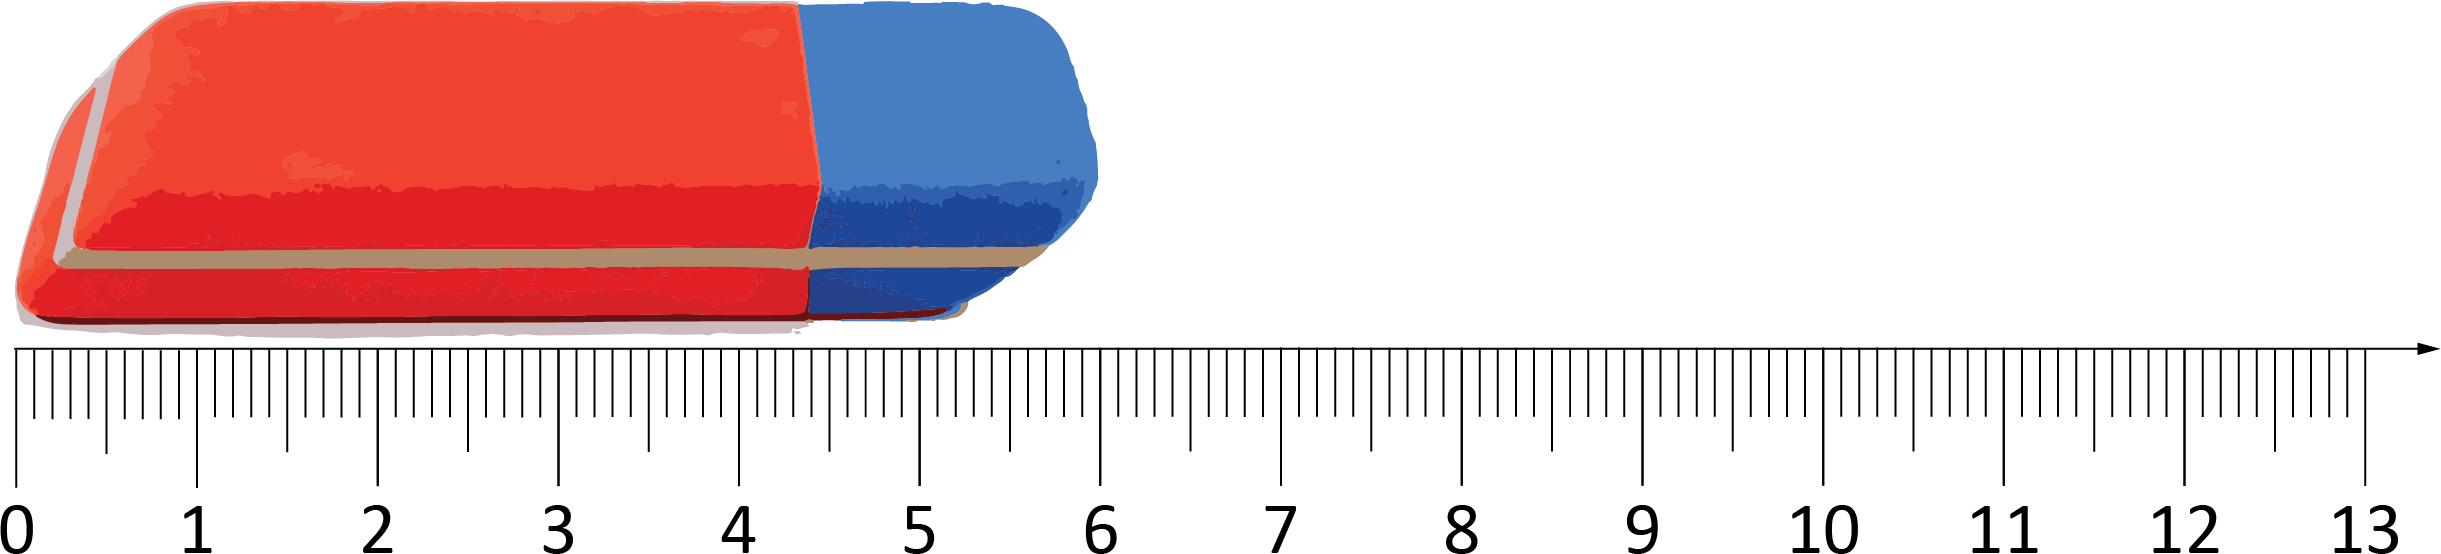
\includegraphics[width=0.6\textwidth]{./media/image43.png}
\end{center}

\item O apontador mede \reduline{4 cm.\hfill}

\begin{center}
\noindent
\includegraphics[width=0.6\textwidth]{./media/image44.png}
\end{center}

\item A tesoura mede \reduline{11 cm.\hfill}

\begin{center}
\noindent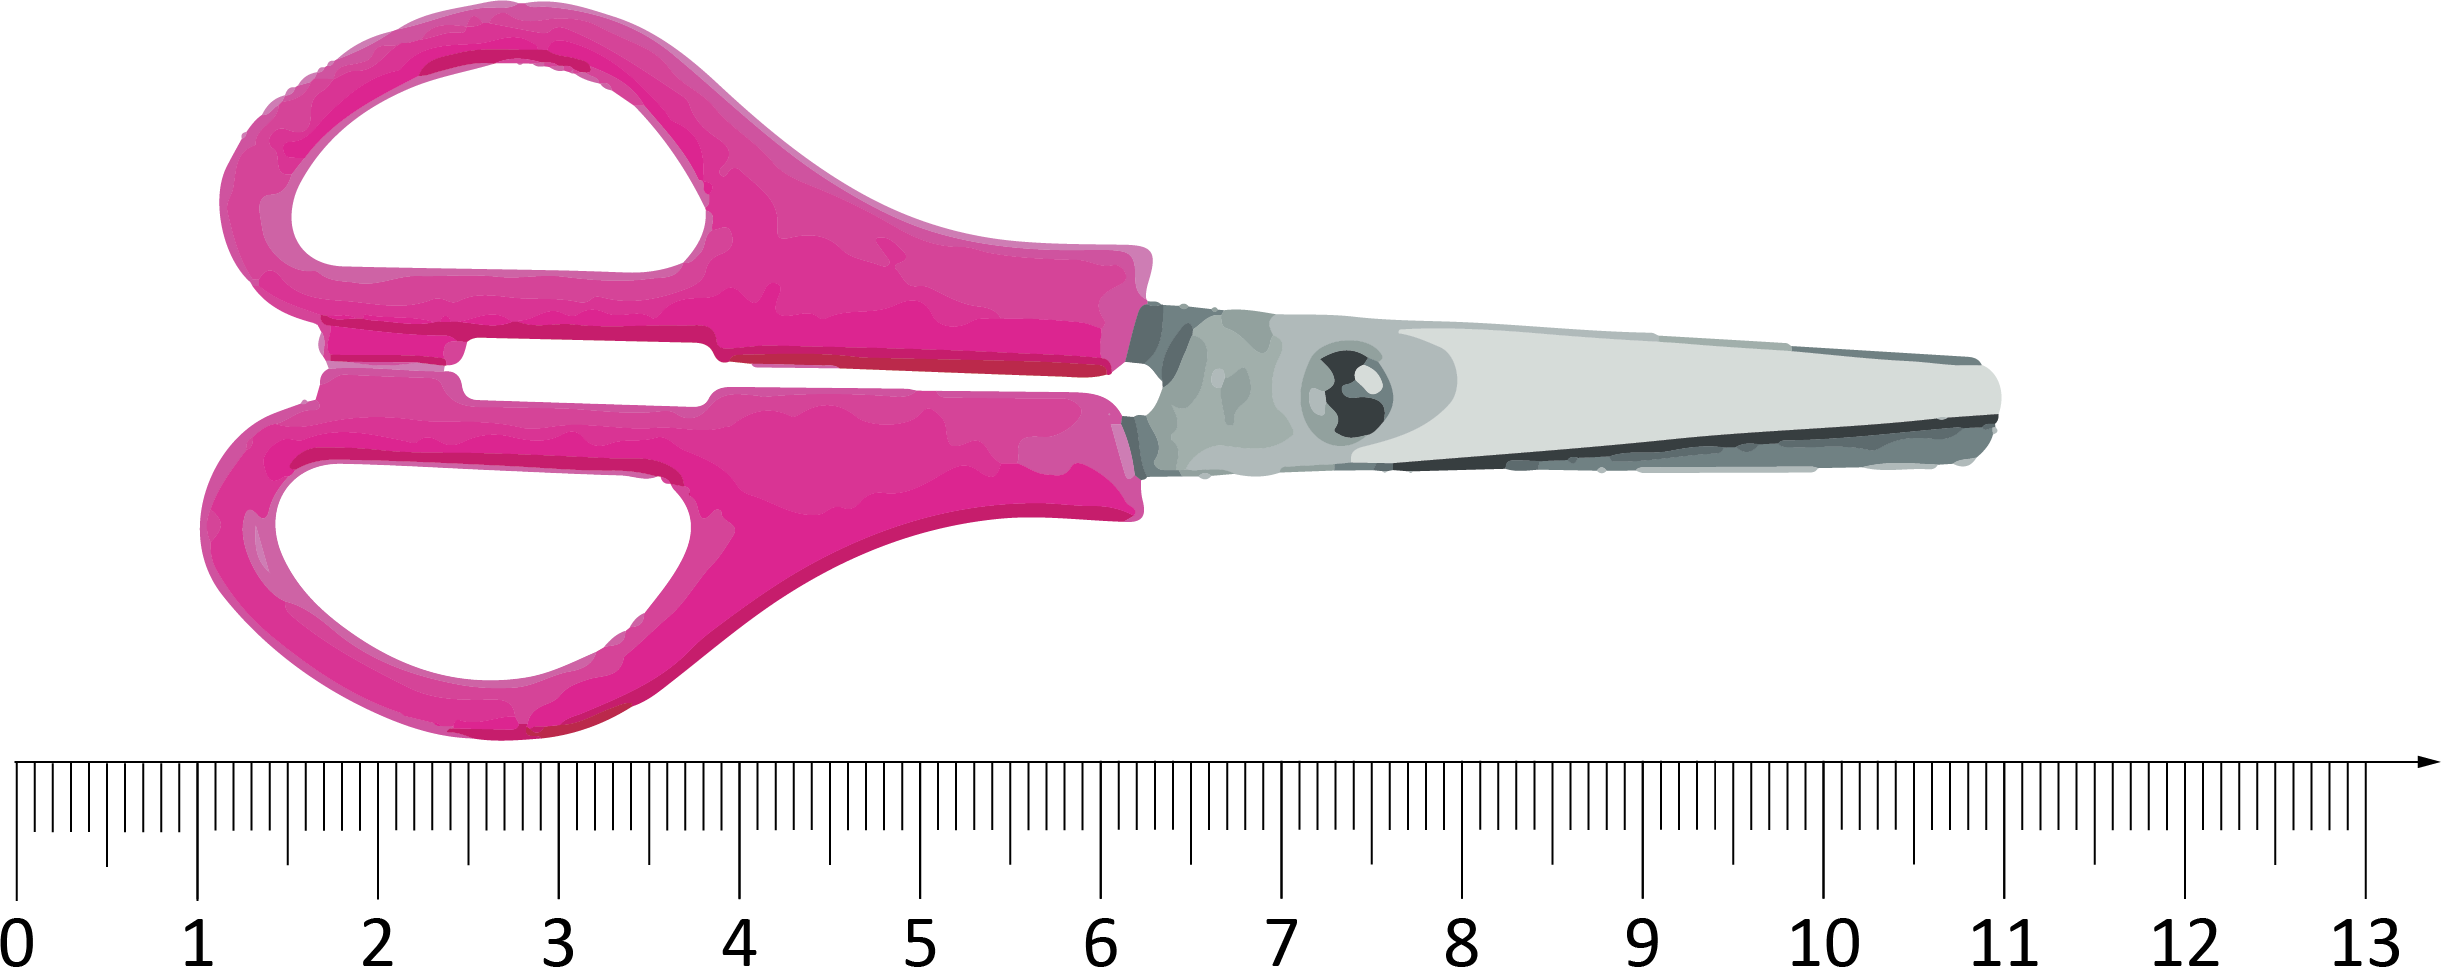
\includegraphics[width=0.6\textwidth]{./media/image45.png}
\end{center}
\end{escolha}

%\coment{Vale a pena explorar bastante essa questão de medir com o auxílio da reta numérica, principalmente quando o início não é no zero. Esse conceito é muito útil para entendimento de assuntos que virão em outros anos e trabalhar bastante agora pode ajudar muito o aluno em anos posteriores.}

\pagebreak
\num{5} Débora decidiu estimar a medida do seu lápis com sua borracha.

\begin{figure}[htpb!]
\centering
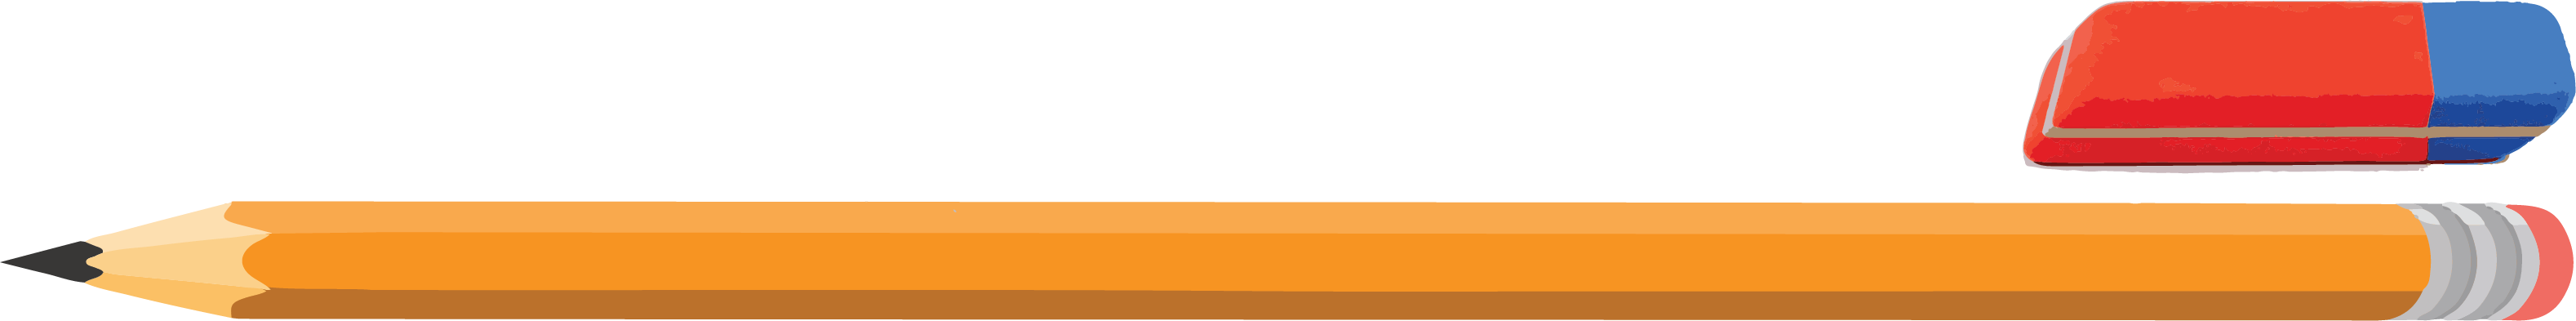
\includegraphics[width=.5\textwidth]{./media/image46.png}
\end{figure}

Quantas borrachas, aproximadamente, mede o lápis de Débora, considerando a figura dada?

\reduline{ Por comparação, pode-se estimar que no comprimento do lápis cabem cerca de 4 a 5 borrachas, conforme a figura dada.\hfill}
\linhas{2}

\num{6} Um dos brinquedos do parque de diversões permanente de uma cidade proíbe
que crianças com altura menor que 1,30 m possam brincar nessa
atração. Manoel mediu sua altura e ele está com 93 cm. Quanto ele
precisa crescer para poder realizar seu sonho de andar nesse brinquedo?
\reduline{1,30 m = 130 cm; 130 -- 93 = 33 cm. Portanto, ele ainda precisará crescer 33 cm para poder usar o brinquedo.\hfill}
\linhas{2}

\num{7} Roberto está com sintomas de dor de garganta, e sua mãe o levou ao
médico. Quando chegou ao consultório, sua temperatura foi medida, como indicado na fotografia a seguir.

\begin{figure}[htpb!]
\centering
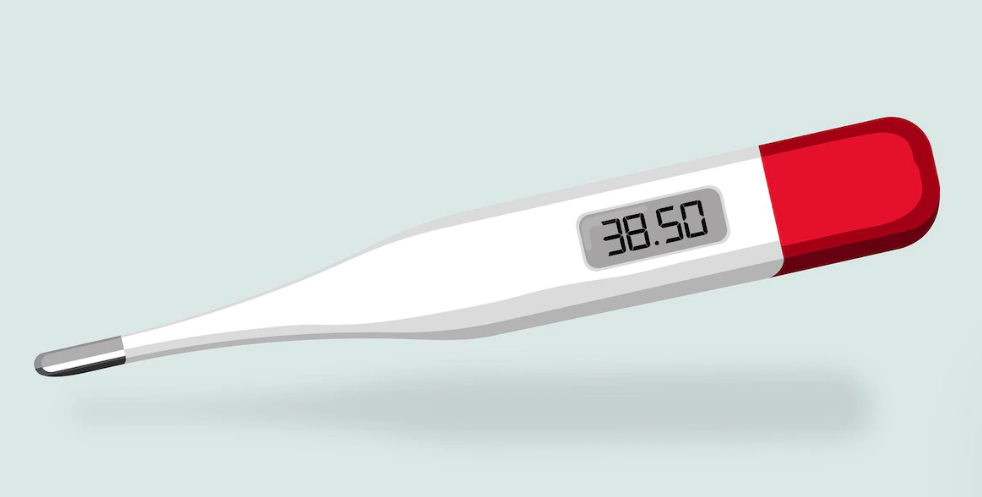
\includegraphics[width=.5\textwidth]{./media/image47.png}
\end{figure}

\begin{escolha}
\item Analisando a imagem do termômetro, qual a temperatura de Roberto nesse instante?
\reduline{38,5º C.\hfill}
\end{escolha}

\num{8} O pai de Arthur encomendou 24 garrafas de
refrigerante para a festa de aniversário do filho. Dessas garrafas, 10 tinham capacidade de 3 litros cada uma delas. As demais garrafas tinham capacidade de 2 litros cada. Com base nessas
informações, responda ao que se pede a seguir.

\begin{figure}[htpb!]
\centering
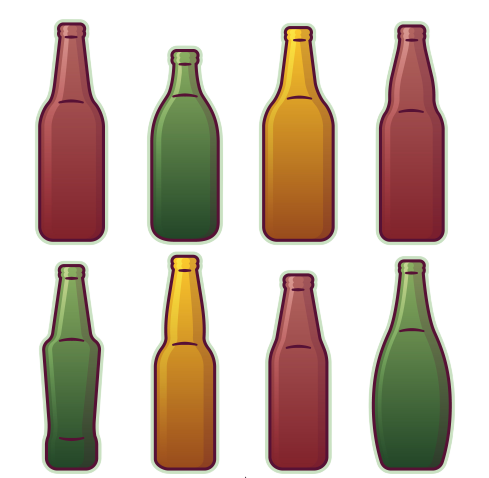
\includegraphics[width=.6\textwidth]{./media/image47a.png}
\end{figure}

\begin{escolha}
\item Qual a quantidade, em mililitros, encomendada pelo pai de Arthur?
\reduline{(10 x 3) + (14 x 2) = 30 + 28 = 58 L = 58.000 ml\hfill}
\linhas{1}

\item Se cada pessoa consumiu exatamente 400 mililitros de refrigerante e
  todo o refrigerante foi consumido durante a festa, quantas pessoas
  foram ao aniversário de Arthur?
\reduline{58.000 : 400 = 145 pessoas compareceram à festa.\hfill}
\linhas{2}
\end{escolha}

\num{9} O comprimento de uma escrivaninha é de 1,6 m. 

\begin{figure}[htpb!]
\centering
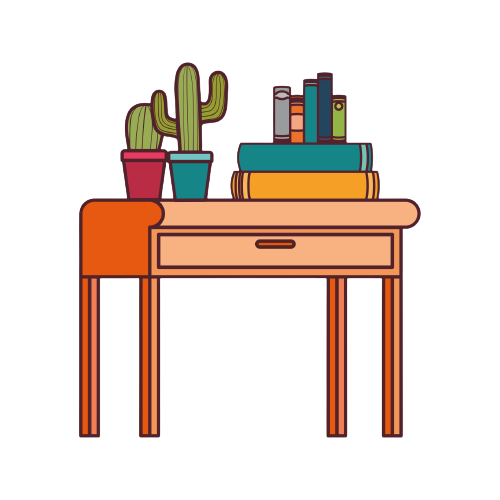
\includegraphics[width=.5\textwidth]{./media/image47b.png}
\end{figure}

\begin{escolha}
\item Quantos palmos,
aproximadamente, mede a escrivaninha se, em média, um palmo tem 23 cm?
\reduline{1,6 m = 160 cm; 160 : 23 = 6,95 palmos. Aproximadamente 7 palmos.\hfill}\linhas{2}
\end{escolha}

\num{10} Os episódios de uma série de televisão têm 45 minutos de duração.
Se Jorge terminou de assistir a um episódio às 17 horas, qual foi o
horário em que ele começou a assistir ao episódio, considerando que não houve interrupções?
\reduline{Jorge começou a assistir ao episódio às 16h15.\hfill}\linhas{1}
\linhas{2} 

\pagebreak
\section*{Treino}

\num{1} Reinaldo foi contratado por uma empresa que exige que se cumpra os horários exatamente como mostra o contrato. No período da manhã, ele deve
cumprir 4 horas e 30 minutos de trabalho. Qual será o horário que
Reinaldo sairá para almoçar?

\begin{longtable}[]{@{}lll@{}}
\toprule
& \textbf{Entrada} & \textbf{Saída}\tabularnewline
\midrule
\endhead
\hline
\textbf{Manhã} & 8:00 & ?\tabularnewline
\hline
\textbf{Tarde} & 14:00 & 17:30\tabularnewline
\hline
\bottomrule
\end{longtable}

\begin{escolha}
\begin{multicols}{2}
% Conteúdo da primeira coluna

\item 11h00.

\item 11h30.
\end{multicols}

% Conteúdo entre as duas colunas

\begin{multicols}{2}
% Conteúdo da segunda coluna

\item 12h00.

\item 12h30.
\end{multicols}
\end{escolha}


\num{2} Júlia está com tosse, e sua avó preparou para ela um chá de menta com mel, ótimo para resolver o problema. A avó colocou o chá na geladeira em garrafinhas de 500 mL. Se Júlia tomar um copinho de 40 mL, 4 vezes ao dia, por dez dias, quantas garrafinhas precisarão ser preparadas pela avó?

\begin{escolha}
\begin{multicols}{2}
% Conteúdo da primeira coluna

\item 1.

\item 2.
\end{multicols}

% Conteúdo entre as duas colunas

\begin{multicols}{2}
% Conteúdo da segunda coluna

\item 3.

\item 4.
\end{multicols}
\end{escolha}


\num{3} Luana foi visitar sua avó, que mora em outro estado. Seu voo
saiu do aeroporto às 8 horas e 15 minutos e chegou ao seu destino às 11
horas e 30 minutos. Calcule o tempo de duração do voo.

\begin{escolha}
\begin{multicols}{2}
% Conteúdo da primeira coluna

\item 3 horas e 15 minutos.

\item 2 horas.
\end{multicols}

% Conteúdo entre as duas colunas

\begin{multicols}{2}
% Conteúdo da segunda coluna

\item 2 horas e 45 minutos.

\item 3 horas e 50 minutos.
\end{multicols}  
\end{escolha}

